\documentclass[12pt]{amsart}
\pagestyle{plain}

\usepackage{amsthm, setspace, framed, url, hyperref, lscape}
\usepackage[none]{hyphenat}
\usepackage[pdftex]{graphicx}
\usepackage{enumerate}
\usepackage{tikz}
\usepackage{courier}
\makeatletter
\def\@settitle{\begin{center}%
  \baselineskip14\p@\relax
  \bfseries
  \uppercasenonmath\@title
  \@title
  \ifx\@subtitle\@empty\else
     \\[1ex]\uppercasenonmath\@subtitle
     \footnotesize\mdseries\@subtitle
  \fi
  \end{center}%
}
\def\subtitle#1{\gdef\@subtitle{#1}}
\def\@subtitle{}
\makeatother

\setlength{\textwidth}{6.0in}
\setlength{\textheight}{8.8in}
\setlength{\oddsidemargin}{0.25in}
\setlength{\evensidemargin}{0.25in}
\setlength{\topmargin}{0in}

\theoremstyle{plain}
\newtheorem{thm}{Theorem}[section]
\newtheorem{lem}[thm]{Lemma}
\newtheorem*{cor}{Corollary}
\newtheorem{quest}{Question}

\theoremstyle{definition}
\newtheorem*{defn}{Definition}
\newtheorem*{ex}{Example}

\theoremstyle{remark}
\newtheorem*{rem}{Remark}
\newtheorem*{note}{Note}
\newtheorem{case}{Case}

\newcommand{\R}{\mathbb{R}}
\newcommand{\Z}{\mathbb{Z}}
\newcommand{\C}{\mathbb{C}}
\newcommand{\N}{\mathbb{N}}
\newcommand{\QQ}{\mathbb{Q}}
\newcommand{\Rnn}{\R^{n\times n}} 
\newcommand{\Rn}{\R^{n}} 

\newcommand{\bx}{{\bf x}}
\newcommand{\bv}{{\bf v}}
\newcommand{\bw}{{\bf w}}
\newcommand{\bu}{{\bf u}}

\newcommand{\bit}{\begin{itemize}}
\newcommand{\eit}{\end{itemize}}
\newcommand{\ben}{\begin{enumerate}}
\newcommand{\een}{\end{enumerate}}
\newcommand{\bea}{\begin{eqnarray*}}
\newcommand{\eea}{\end{eqnarray*}}
\newcommand{\bpf}{\begin{proof}}
\newcommand{\epf}{\end{proof}\ms}
\newcommand{\bthm}{\begin{thm}}
\newcommand{\ethm}{\end{thm}}
\newcommand{\bdefn}{\begin{defn}}
\newcommand{\edefn}{\end{defn}}
\newcommand{\bex}{\begin{ex}}
\newcommand{\eex}{\end{ex}}
\newcommand{\bde}{\begin{description}}
\newcommand{\ede}{\end{description}}
\newcommand{\bcen}{\begin{center}}
\newcommand{\ecen}{\end{center}}
\newcommand{\bq}{\begin{quest}}
\newcommand{\eq}{\end{quest}}

\newcommand*\circled[1]{\tikz[baseline=(char.base)]{
            \node[shape=circle,draw,inner sep=2pt] (char) {#1};}}

\begin{document}

\onehalfspacing

\title[]{Cryptography Handout 02}
\subtitle{Vigen\`{e}re Cipher}
\maketitle

\section{Number and Letter Correspondence ($\bmod 26$)}
\bcen
\begin{tabular}{|p{.25in}|p{.25in}|p{.25in}|p{.25in}|p{.25in}|p{.25in}|p{.25in}|p{.25in}|p{.25in}|p{.25in}|p{.25in}|p{.25in}|p{.25in}|}\hline
a & b & c & d & e & f & g & h & i & j & k & l & m\\
0 & 1 & 2 & 3 & 4 & 5 & 6 & 7 & 8 & 9 & 10 & 11 & 12 \\ \hline
n & o & p & q & r & s & t & u & v & w & x & y & z\\
13 &14 & 15 & 16 & 17 & 18 & 19 & 20 & 21 & 22 & 23 & 24 & 25\\ \hline
\end{tabular}
\ecen

\section{Vigen\`{e}re Table}
\bcen
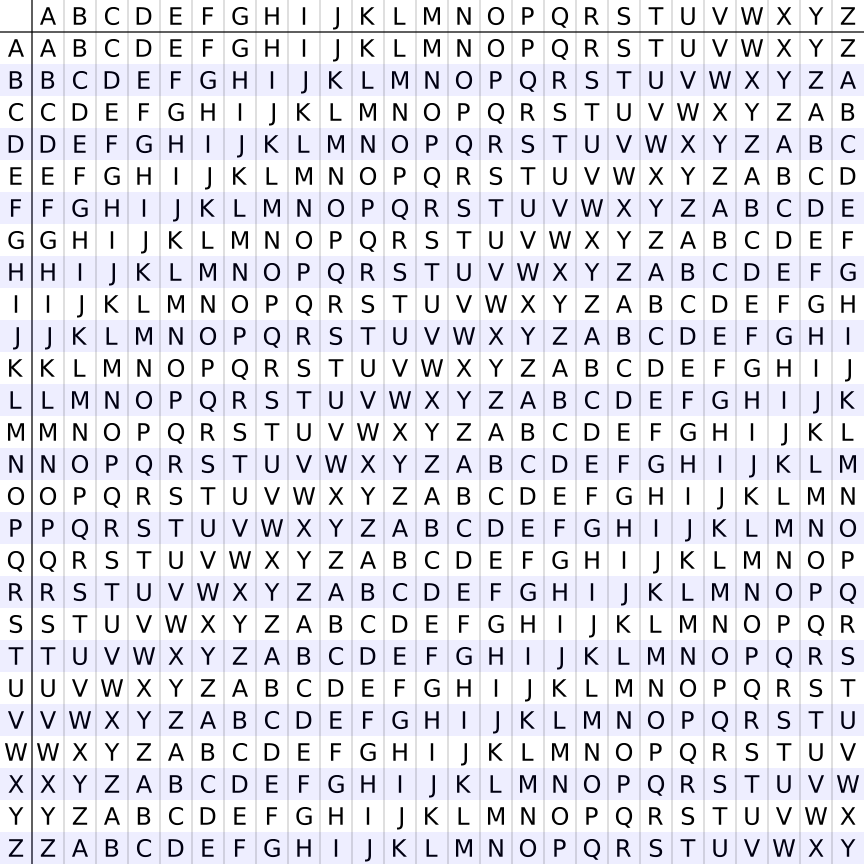
\includegraphics[width=5in]{Vigenere.png}
\url{https://en.wikipedia.org/wiki/Vigen%C3%A8re_cipher}
\ecen

\section{Frequencies of Letters in English}

\bcen
\begin{tabular}{lllllllllllll} \hline
a & b & c & d & e & f & g & h & i & j & k & l & m\\
.082 & .015 & .028 & .043 & .127 & .022 & .020 & .061 & .070 & .002 & .008 & .040 & .024\\ \hline
n & o & p & q & r & s & t & u & v & w & x & y & z\\ 
.067 & .075 & .019 & .001 & .060 & .063 & .091 & .028 & .010 & .023 & .001 & .020 & .001\\ \hline
\end{tabular}
\ecen
 
\section{Vigen\`{e}re Example}
\noindent (From 2.3 in Trappe and Washington)  \\
\texttt{\circled{V}VHQW\circled{V}VRHM\circled{U}SGJG\circled{T}HKIH\circled{T}SSEJ\circled{C}HLSF\circled{C}BGVW\circled{C}RLRY\circled{Q}TFSV\circled{G}AHW}\\
\texttt{K\circled{C}UHWA\circled{U}GLQH\circled{N}SLRL\circled{J}SHBL\circled{T}SPIS\circled{P}RDXL\circled{J}SVEE\circled{G}HLQW\circled{K}ASSK\circled{U}WE}\\
\texttt{PW\circled{Q}TWVS\circled{P}GOEL\circled{K}CQYF\circled{N}SVWL\circled{J}SNIQ\circled{K}GNRG\circled{Y}BWLW\circled{G}OVIO\circled{K}HKAZ\circled{K}Q}\\
\texttt{KXZ\circled{G}YHCE\circled{C}MEIU\circled{J}OQKW\circled{F}WVEF\circled{Q}HKIJ\circled{R}CLRL\circled{K}BIEN\circled{Q}FRJL\circled{J}SDHG\circled{R}}\\
\texttt{HLSF\circled{Q}TWLA\circled{U}QRHW\circled{D}MWLG\circled{U}SGIK\circled{K}FLRY\circled{V}CWVS\circled{P}GPML\circled{K}ASSJ\circled{V}OQXE}\\
\texttt{\circled{G}GVEY\circled{G}GZML\circled{J}CXXL\circled{J}SVPA\circled{I}VWIK\circled{V}RDRY\circled{G}FRJL\circled{J}SLVE\circled{G}GVEY\circled{G}GEI}\\
\texttt{A\circled{P}UUIS\circled{F}PBTG\circled{N}WWMU\circled{C}ZRVT\circled{W}GLRW\circled{U}GUMN\circled{C}ZVIL\circled{E}}\\

See Frequency Analysis code.

\subsection{Key Length} \label{keylength}
\ben[1.]
	\item Take the ciphertext and write it on two strips of paper.
	\item Put one strip of paper above the other but displaced by a certain number of places.
	\item Mark the number of times a letter and the one below it are the same.
	\item Count the number of coincidences.
\een

See last page for printout.

\subsection{Finding the Key: Method 2 (in text)}
For $i = 1$ to $n$,
\ben[1.]
	\item Compute frequencies of the letters in positions $i \bmod n$, and form the vector $\vec{W}$.
	\item For $j = 1$ to $25$, compute $\vec{W} \cdot \vec{A}_j$.
	\item Let $k_i = j_0$ give the maximum value of $\vec{W} \cdot \vec{A}_j$.
\een
The key is probably $\{k_1,k_2,k_3, \cdots, k_n\}$.


\newpage
\begin{landscape}
\section{Vigen\`{e}re Key Length Example}
Print the following out, and cut into two strips.  Then follow the instructions from Section \ref{keylength}.\\
\vspace{.5in}

{\fontsize{.65in}{.5in}\selectfont \texttt{VVHQWVVRHMUSGHGTHKIHT...}}
\vspace{.5in}

{\fontsize{.65in}{.5in}\selectfont \texttt{VVHQWVVRHMUSGHGTHKIHT...}}

\end{landscape}
	
\end{document}